% Created by tikzDevice version 0.12.6 on 2025-02-16 17:48:18
% !TEX encoding = UTF-8 Unicode
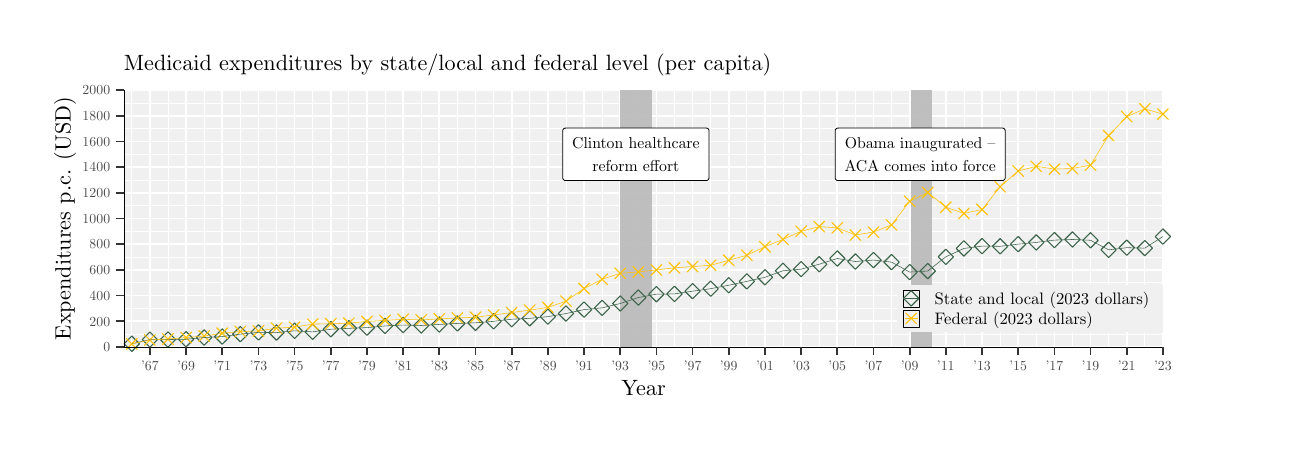
\begin{tikzpicture}[x=1pt,y=1pt]
\definecolor{fillColor}{RGB}{255,255,255}
\path[use as bounding box,fill=fillColor,fill opacity=0.00] (0,0) rectangle (455.30,144.54);
\begin{scope}
\path[clip] (  0.00,  0.00) rectangle (455.30,144.54);
\definecolor{drawColor}{RGB}{255,255,255}
\definecolor{fillColor}{RGB}{255,255,255}

\path[draw=drawColor,line width= 0.6pt,line join=round,line cap=round,fill=fillColor] (  0.00,  0.00) rectangle (455.30,144.54);
\end{scope}
\begin{scope}
\path[clip] (  0.00,  0.00) rectangle (455.30,144.54);
\definecolor{fillColor}{gray}{0.94}

\path[fill=fillColor] ( 34.76, 29.18) rectangle (410.30,121.98);
\definecolor{drawColor}{RGB}{255,255,255}

\path[draw=drawColor,line width= 0.3pt,line join=round] ( 34.76, 33.82) --
	(410.30, 33.82);

\path[draw=drawColor,line width= 0.3pt,line join=round] ( 34.76, 43.10) --
	(410.30, 43.10);

\path[draw=drawColor,line width= 0.3pt,line join=round] ( 34.76, 52.38) --
	(410.30, 52.38);

\path[draw=drawColor,line width= 0.3pt,line join=round] ( 34.76, 61.66) --
	(410.30, 61.66);

\path[draw=drawColor,line width= 0.3pt,line join=round] ( 34.76, 70.94) --
	(410.30, 70.94);

\path[draw=drawColor,line width= 0.3pt,line join=round] ( 34.76, 80.22) --
	(410.30, 80.22);

\path[draw=drawColor,line width= 0.3pt,line join=round] ( 34.76, 89.50) --
	(410.30, 89.50);

\path[draw=drawColor,line width= 0.3pt,line join=round] ( 34.76, 98.78) --
	(410.30, 98.78);

\path[draw=drawColor,line width= 0.3pt,line join=round] ( 34.76,108.06) --
	(410.30,108.06);

\path[draw=drawColor,line width= 0.3pt,line join=round] ( 34.76,117.34) --
	(410.30,117.34);

\path[draw=drawColor,line width= 0.3pt,line join=round] ( 37.63, 29.18) --
	( 37.63,121.98);

\path[draw=drawColor,line width= 0.3pt,line join=round] ( 50.70, 29.18) --
	( 50.70,121.98);

\path[draw=drawColor,line width= 0.3pt,line join=round] ( 63.77, 29.18) --
	( 63.77,121.98);

\path[draw=drawColor,line width= 0.3pt,line join=round] ( 76.85, 29.18) --
	( 76.85,121.98);

\path[draw=drawColor,line width= 0.3pt,line join=round] ( 89.92, 29.18) --
	( 89.92,121.98);

\path[draw=drawColor,line width= 0.3pt,line join=round] (102.99, 29.18) --
	(102.99,121.98);

\path[draw=drawColor,line width= 0.3pt,line join=round] (116.07, 29.18) --
	(116.07,121.98);

\path[draw=drawColor,line width= 0.3pt,line join=round] (129.14, 29.18) --
	(129.14,121.98);

\path[draw=drawColor,line width= 0.3pt,line join=round] (142.21, 29.18) --
	(142.21,121.98);

\path[draw=drawColor,line width= 0.3pt,line join=round] (155.29, 29.18) --
	(155.29,121.98);

\path[draw=drawColor,line width= 0.3pt,line join=round] (168.36, 29.18) --
	(168.36,121.98);

\path[draw=drawColor,line width= 0.3pt,line join=round] (181.43, 29.18) --
	(181.43,121.98);

\path[draw=drawColor,line width= 0.3pt,line join=round] (194.51, 29.18) --
	(194.51,121.98);

\path[draw=drawColor,line width= 0.3pt,line join=round] (207.58, 29.18) --
	(207.58,121.98);

\path[draw=drawColor,line width= 0.3pt,line join=round] (220.65, 29.18) --
	(220.65,121.98);

\path[draw=drawColor,line width= 0.3pt,line join=round] (233.73, 29.18) --
	(233.73,121.98);

\path[draw=drawColor,line width= 0.3pt,line join=round] (246.80, 29.18) --
	(246.80,121.98);

\path[draw=drawColor,line width= 0.3pt,line join=round] (259.87, 29.18) --
	(259.87,121.98);

\path[draw=drawColor,line width= 0.3pt,line join=round] (272.95, 29.18) --
	(272.95,121.98);

\path[draw=drawColor,line width= 0.3pt,line join=round] (286.02, 29.18) --
	(286.02,121.98);

\path[draw=drawColor,line width= 0.3pt,line join=round] (299.09, 29.18) --
	(299.09,121.98);

\path[draw=drawColor,line width= 0.3pt,line join=round] (312.17, 29.18) --
	(312.17,121.98);

\path[draw=drawColor,line width= 0.3pt,line join=round] (325.24, 29.18) --
	(325.24,121.98);

\path[draw=drawColor,line width= 0.3pt,line join=round] (338.31, 29.18) --
	(338.31,121.98);

\path[draw=drawColor,line width= 0.3pt,line join=round] (351.39, 29.18) --
	(351.39,121.98);

\path[draw=drawColor,line width= 0.3pt,line join=round] (364.46, 29.18) --
	(364.46,121.98);

\path[draw=drawColor,line width= 0.3pt,line join=round] (377.53, 29.18) --
	(377.53,121.98);

\path[draw=drawColor,line width= 0.3pt,line join=round] (390.61, 29.18) --
	(390.61,121.98);

\path[draw=drawColor,line width= 0.3pt,line join=round] (403.68, 29.18) --
	(403.68,121.98);

\path[draw=drawColor,line width= 0.6pt,line join=round] ( 34.76, 29.18) --
	(410.30, 29.18);

\path[draw=drawColor,line width= 0.6pt,line join=round] ( 34.76, 38.46) --
	(410.30, 38.46);

\path[draw=drawColor,line width= 0.6pt,line join=round] ( 34.76, 47.74) --
	(410.30, 47.74);

\path[draw=drawColor,line width= 0.6pt,line join=round] ( 34.76, 57.02) --
	(410.30, 57.02);

\path[draw=drawColor,line width= 0.6pt,line join=round] ( 34.76, 66.30) --
	(410.30, 66.30);

\path[draw=drawColor,line width= 0.6pt,line join=round] ( 34.76, 75.58) --
	(410.30, 75.58);

\path[draw=drawColor,line width= 0.6pt,line join=round] ( 34.76, 84.86) --
	(410.30, 84.86);

\path[draw=drawColor,line width= 0.6pt,line join=round] ( 34.76, 94.14) --
	(410.30, 94.14);

\path[draw=drawColor,line width= 0.6pt,line join=round] ( 34.76,103.42) --
	(410.30,103.42);

\path[draw=drawColor,line width= 0.6pt,line join=round] ( 34.76,112.70) --
	(410.30,112.70);

\path[draw=drawColor,line width= 0.6pt,line join=round] ( 34.76,121.98) --
	(410.30,121.98);

\path[draw=drawColor,line width= 0.6pt,line join=round] ( 44.16, 29.18) --
	( 44.16,121.98);

\path[draw=drawColor,line width= 0.6pt,line join=round] ( 57.24, 29.18) --
	( 57.24,121.98);

\path[draw=drawColor,line width= 0.6pt,line join=round] ( 70.30, 29.18) --
	( 70.30,121.98);

\path[draw=drawColor,line width= 0.6pt,line join=round] ( 83.39, 29.18) --
	( 83.39,121.98);

\path[draw=drawColor,line width= 0.6pt,line join=round] ( 96.45, 29.18) --
	( 96.45,121.98);

\path[draw=drawColor,line width= 0.6pt,line join=round] (109.53, 29.18) --
	(109.53,121.98);

\path[draw=drawColor,line width= 0.6pt,line join=round] (122.60, 29.18) --
	(122.60,121.98);

\path[draw=drawColor,line width= 0.6pt,line join=round] (135.68, 29.18) --
	(135.68,121.98);

\path[draw=drawColor,line width= 0.6pt,line join=round] (148.74, 29.18) --
	(148.74,121.98);

\path[draw=drawColor,line width= 0.6pt,line join=round] (161.83, 29.18) --
	(161.83,121.98);

\path[draw=drawColor,line width= 0.6pt,line join=round] (174.89, 29.18) --
	(174.89,121.98);

\path[draw=drawColor,line width= 0.6pt,line join=round] (187.97, 29.18) --
	(187.97,121.98);

\path[draw=drawColor,line width= 0.6pt,line join=round] (201.04, 29.18) --
	(201.04,121.98);

\path[draw=drawColor,line width= 0.6pt,line join=round] (214.12, 29.18) --
	(214.12,121.98);

\path[draw=drawColor,line width= 0.6pt,line join=round] (227.18, 29.18) --
	(227.18,121.98);

\path[draw=drawColor,line width= 0.6pt,line join=round] (240.27, 29.18) --
	(240.27,121.98);

\path[draw=drawColor,line width= 0.6pt,line join=round] (253.33, 29.18) --
	(253.33,121.98);

\path[draw=drawColor,line width= 0.6pt,line join=round] (266.41, 29.18) --
	(266.41,121.98);

\path[draw=drawColor,line width= 0.6pt,line join=round] (279.48, 29.18) --
	(279.48,121.98);

\path[draw=drawColor,line width= 0.6pt,line join=round] (292.56, 29.18) --
	(292.56,121.98);

\path[draw=drawColor,line width= 0.6pt,line join=round] (305.62, 29.18) --
	(305.62,121.98);

\path[draw=drawColor,line width= 0.6pt,line join=round] (318.71, 29.18) --
	(318.71,121.98);

\path[draw=drawColor,line width= 0.6pt,line join=round] (331.77, 29.18) --
	(331.77,121.98);

\path[draw=drawColor,line width= 0.6pt,line join=round] (344.85, 29.18) --
	(344.85,121.98);

\path[draw=drawColor,line width= 0.6pt,line join=round] (357.92, 29.18) --
	(357.92,121.98);

\path[draw=drawColor,line width= 0.6pt,line join=round] (371.00, 29.18) --
	(371.00,121.98);

\path[draw=drawColor,line width= 0.6pt,line join=round] (384.06, 29.18) --
	(384.06,121.98);

\path[draw=drawColor,line width= 0.6pt,line join=round] (397.15, 29.18) --
	(397.15,121.98);

\path[draw=drawColor,line width= 0.6pt,line join=round] (410.21, 29.18) --
	(410.21,121.98);
\definecolor{drawColor}{RGB}{190,190,190}

\path[draw=drawColor,line width= 0.6pt,line join=round] ( -1.60, 29.18) -- ( -1.60,121.98);
\definecolor{fillColor}{RGB}{190,190,190}

\path[fill=fillColor,fill opacity=0.01] (214.12, 29.18) rectangle (225.45,121.98);

\path[fill=fillColor,fill opacity=0.01] (214.12, 29.18) rectangle (225.45,121.98);

\path[fill=fillColor,fill opacity=0.01] (214.12, 29.18) rectangle (225.45,121.98);

\path[fill=fillColor,fill opacity=0.01] (214.12, 29.18) rectangle (225.45,121.98);

\path[fill=fillColor,fill opacity=0.01] (214.12, 29.18) rectangle (225.45,121.98);

\path[fill=fillColor,fill opacity=0.01] (214.12, 29.18) rectangle (225.45,121.98);

\path[fill=fillColor,fill opacity=0.01] (214.12, 29.18) rectangle (225.45,121.98);

\path[fill=fillColor,fill opacity=0.01] (214.12, 29.18) rectangle (225.45,121.98);

\path[fill=fillColor,fill opacity=0.01] (214.12, 29.18) rectangle (225.45,121.98);

\path[fill=fillColor,fill opacity=0.01] (214.12, 29.18) rectangle (225.45,121.98);

\path[fill=fillColor,fill opacity=0.01] (214.12, 29.18) rectangle (225.45,121.98);

\path[fill=fillColor,fill opacity=0.01] (214.12, 29.18) rectangle (225.45,121.98);

\path[fill=fillColor,fill opacity=0.01] (214.12, 29.18) rectangle (225.45,121.98);

\path[fill=fillColor,fill opacity=0.01] (214.12, 29.18) rectangle (225.45,121.98);

\path[fill=fillColor,fill opacity=0.01] (214.12, 29.18) rectangle (225.45,121.98);

\path[fill=fillColor,fill opacity=0.01] (214.12, 29.18) rectangle (225.45,121.98);

\path[fill=fillColor,fill opacity=0.01] (214.12, 29.18) rectangle (225.45,121.98);

\path[fill=fillColor,fill opacity=0.01] (214.12, 29.18) rectangle (225.45,121.98);

\path[fill=fillColor,fill opacity=0.01] (214.12, 29.18) rectangle (225.45,121.98);

\path[fill=fillColor,fill opacity=0.01] (214.12, 29.18) rectangle (225.45,121.98);

\path[fill=fillColor,fill opacity=0.01] (214.12, 29.18) rectangle (225.45,121.98);

\path[fill=fillColor,fill opacity=0.01] (214.12, 29.18) rectangle (225.45,121.98);

\path[fill=fillColor,fill opacity=0.01] (214.12, 29.18) rectangle (225.45,121.98);

\path[fill=fillColor,fill opacity=0.01] (214.12, 29.18) rectangle (225.45,121.98);

\path[fill=fillColor,fill opacity=0.01] (214.12, 29.18) rectangle (225.45,121.98);

\path[fill=fillColor,fill opacity=0.01] (214.12, 29.18) rectangle (225.45,121.98);

\path[fill=fillColor,fill opacity=0.01] (214.12, 29.18) rectangle (225.45,121.98);

\path[fill=fillColor,fill opacity=0.01] (214.12, 29.18) rectangle (225.45,121.98);

\path[fill=fillColor,fill opacity=0.01] (214.12, 29.18) rectangle (225.45,121.98);

\path[fill=fillColor,fill opacity=0.01] (214.12, 29.18) rectangle (225.45,121.98);

\path[fill=fillColor,fill opacity=0.01] (214.12, 29.18) rectangle (225.45,121.98);

\path[fill=fillColor,fill opacity=0.01] (214.12, 29.18) rectangle (225.45,121.98);

\path[fill=fillColor,fill opacity=0.01] (214.12, 29.18) rectangle (225.45,121.98);

\path[fill=fillColor,fill opacity=0.01] (214.12, 29.18) rectangle (225.45,121.98);

\path[fill=fillColor,fill opacity=0.01] (214.12, 29.18) rectangle (225.45,121.98);

\path[fill=fillColor,fill opacity=0.01] (214.12, 29.18) rectangle (225.45,121.98);

\path[fill=fillColor,fill opacity=0.01] (214.12, 29.18) rectangle (225.45,121.98);

\path[fill=fillColor,fill opacity=0.01] (214.12, 29.18) rectangle (225.45,121.98);

\path[fill=fillColor,fill opacity=0.01] (214.12, 29.18) rectangle (225.45,121.98);

\path[fill=fillColor,fill opacity=0.01] (214.12, 29.18) rectangle (225.45,121.98);

\path[fill=fillColor,fill opacity=0.01] (214.12, 29.18) rectangle (225.45,121.98);

\path[fill=fillColor,fill opacity=0.01] (214.12, 29.18) rectangle (225.45,121.98);

\path[fill=fillColor,fill opacity=0.01] (214.12, 29.18) rectangle (225.45,121.98);

\path[fill=fillColor,fill opacity=0.01] (214.12, 29.18) rectangle (225.45,121.98);

\path[fill=fillColor,fill opacity=0.01] (214.12, 29.18) rectangle (225.45,121.98);

\path[fill=fillColor,fill opacity=0.01] (214.12, 29.18) rectangle (225.45,121.98);

\path[fill=fillColor,fill opacity=0.01] (214.12, 29.18) rectangle (225.45,121.98);

\path[fill=fillColor,fill opacity=0.01] (214.12, 29.18) rectangle (225.45,121.98);

\path[fill=fillColor,fill opacity=0.01] (214.12, 29.18) rectangle (225.45,121.98);

\path[fill=fillColor,fill opacity=0.01] (214.12, 29.18) rectangle (225.45,121.98);

\path[fill=fillColor,fill opacity=0.01] (214.12, 29.18) rectangle (225.45,121.98);

\path[fill=fillColor,fill opacity=0.01] (214.12, 29.18) rectangle (225.45,121.98);

\path[fill=fillColor,fill opacity=0.01] (214.12, 29.18) rectangle (225.45,121.98);

\path[fill=fillColor,fill opacity=0.01] (214.12, 29.18) rectangle (225.45,121.98);

\path[fill=fillColor,fill opacity=0.01] (214.12, 29.18) rectangle (225.45,121.98);

\path[fill=fillColor,fill opacity=0.01] (214.12, 29.18) rectangle (225.45,121.98);

\path[fill=fillColor,fill opacity=0.01] (214.12, 29.18) rectangle (225.45,121.98);

\path[fill=fillColor,fill opacity=0.01] (214.12, 29.18) rectangle (225.45,121.98);

\path[fill=fillColor,fill opacity=0.01] (214.12, 29.18) rectangle (225.45,121.98);

\path[fill=fillColor,fill opacity=0.01] (214.12, 29.18) rectangle (225.45,121.98);

\path[fill=fillColor,fill opacity=0.01] (214.12, 29.18) rectangle (225.45,121.98);

\path[fill=fillColor,fill opacity=0.01] (214.12, 29.18) rectangle (225.45,121.98);

\path[fill=fillColor,fill opacity=0.01] (214.12, 29.18) rectangle (225.45,121.98);

\path[fill=fillColor,fill opacity=0.01] (214.12, 29.18) rectangle (225.45,121.98);

\path[fill=fillColor,fill opacity=0.01] (319.05, 29.18) rectangle (326.69,121.98);

\path[fill=fillColor,fill opacity=0.01] (319.05, 29.18) rectangle (326.69,121.98);

\path[fill=fillColor,fill opacity=0.01] (319.05, 29.18) rectangle (326.69,121.98);

\path[fill=fillColor,fill opacity=0.01] (319.05, 29.18) rectangle (326.69,121.98);

\path[fill=fillColor,fill opacity=0.01] (319.05, 29.18) rectangle (326.69,121.98);

\path[fill=fillColor,fill opacity=0.01] (319.05, 29.18) rectangle (326.69,121.98);

\path[fill=fillColor,fill opacity=0.01] (319.05, 29.18) rectangle (326.69,121.98);

\path[fill=fillColor,fill opacity=0.01] (319.05, 29.18) rectangle (326.69,121.98);

\path[fill=fillColor,fill opacity=0.01] (319.05, 29.18) rectangle (326.69,121.98);

\path[fill=fillColor,fill opacity=0.01] (319.05, 29.18) rectangle (326.69,121.98);

\path[fill=fillColor,fill opacity=0.01] (319.05, 29.18) rectangle (326.69,121.98);

\path[fill=fillColor,fill opacity=0.01] (319.05, 29.18) rectangle (326.69,121.98);

\path[fill=fillColor,fill opacity=0.01] (319.05, 29.18) rectangle (326.69,121.98);

\path[fill=fillColor,fill opacity=0.01] (319.05, 29.18) rectangle (326.69,121.98);

\path[fill=fillColor,fill opacity=0.01] (319.05, 29.18) rectangle (326.69,121.98);

\path[fill=fillColor,fill opacity=0.01] (319.05, 29.18) rectangle (326.69,121.98);

\path[fill=fillColor,fill opacity=0.01] (319.05, 29.18) rectangle (326.69,121.98);

\path[fill=fillColor,fill opacity=0.01] (319.05, 29.18) rectangle (326.69,121.98);

\path[fill=fillColor,fill opacity=0.01] (319.05, 29.18) rectangle (326.69,121.98);

\path[fill=fillColor,fill opacity=0.01] (319.05, 29.18) rectangle (326.69,121.98);

\path[fill=fillColor,fill opacity=0.01] (319.05, 29.18) rectangle (326.69,121.98);

\path[fill=fillColor,fill opacity=0.01] (319.05, 29.18) rectangle (326.69,121.98);

\path[fill=fillColor,fill opacity=0.01] (319.05, 29.18) rectangle (326.69,121.98);

\path[fill=fillColor,fill opacity=0.01] (319.05, 29.18) rectangle (326.69,121.98);

\path[fill=fillColor,fill opacity=0.01] (319.05, 29.18) rectangle (326.69,121.98);

\path[fill=fillColor,fill opacity=0.01] (319.05, 29.18) rectangle (326.69,121.98);

\path[fill=fillColor,fill opacity=0.01] (319.05, 29.18) rectangle (326.69,121.98);

\path[fill=fillColor,fill opacity=0.01] (319.05, 29.18) rectangle (326.69,121.98);

\path[fill=fillColor,fill opacity=0.01] (319.05, 29.18) rectangle (326.69,121.98);

\path[fill=fillColor,fill opacity=0.01] (319.05, 29.18) rectangle (326.69,121.98);

\path[fill=fillColor,fill opacity=0.01] (319.05, 29.18) rectangle (326.69,121.98);

\path[fill=fillColor,fill opacity=0.01] (319.05, 29.18) rectangle (326.69,121.98);

\path[fill=fillColor,fill opacity=0.01] (319.05, 29.18) rectangle (326.69,121.98);

\path[fill=fillColor,fill opacity=0.01] (319.05, 29.18) rectangle (326.69,121.98);

\path[fill=fillColor,fill opacity=0.01] (319.05, 29.18) rectangle (326.69,121.98);

\path[fill=fillColor,fill opacity=0.01] (319.05, 29.18) rectangle (326.69,121.98);

\path[fill=fillColor,fill opacity=0.01] (319.05, 29.18) rectangle (326.69,121.98);

\path[fill=fillColor,fill opacity=0.01] (319.05, 29.18) rectangle (326.69,121.98);

\path[fill=fillColor,fill opacity=0.01] (319.05, 29.18) rectangle (326.69,121.98);

\path[fill=fillColor,fill opacity=0.01] (319.05, 29.18) rectangle (326.69,121.98);

\path[fill=fillColor,fill opacity=0.01] (319.05, 29.18) rectangle (326.69,121.98);

\path[fill=fillColor,fill opacity=0.01] (319.05, 29.18) rectangle (326.69,121.98);

\path[fill=fillColor,fill opacity=0.01] (319.05, 29.18) rectangle (326.69,121.98);

\path[fill=fillColor,fill opacity=0.01] (319.05, 29.18) rectangle (326.69,121.98);

\path[fill=fillColor,fill opacity=0.01] (319.05, 29.18) rectangle (326.69,121.98);

\path[fill=fillColor,fill opacity=0.01] (319.05, 29.18) rectangle (326.69,121.98);

\path[fill=fillColor,fill opacity=0.01] (319.05, 29.18) rectangle (326.69,121.98);

\path[fill=fillColor,fill opacity=0.01] (319.05, 29.18) rectangle (326.69,121.98);

\path[fill=fillColor,fill opacity=0.01] (319.05, 29.18) rectangle (326.69,121.98);

\path[fill=fillColor,fill opacity=0.01] (319.05, 29.18) rectangle (326.69,121.98);

\path[fill=fillColor,fill opacity=0.01] (319.05, 29.18) rectangle (326.69,121.98);

\path[fill=fillColor,fill opacity=0.01] (319.05, 29.18) rectangle (326.69,121.98);

\path[fill=fillColor,fill opacity=0.01] (319.05, 29.18) rectangle (326.69,121.98);

\path[fill=fillColor,fill opacity=0.01] (319.05, 29.18) rectangle (326.69,121.98);

\path[fill=fillColor,fill opacity=0.01] (319.05, 29.18) rectangle (326.69,121.98);

\path[fill=fillColor,fill opacity=0.01] (319.05, 29.18) rectangle (326.69,121.98);

\path[fill=fillColor,fill opacity=0.01] (319.05, 29.18) rectangle (326.69,121.98);

\path[fill=fillColor,fill opacity=0.01] (319.05, 29.18) rectangle (326.69,121.98);

\path[fill=fillColor,fill opacity=0.01] (319.05, 29.18) rectangle (326.69,121.98);

\path[fill=fillColor,fill opacity=0.01] (319.05, 29.18) rectangle (326.69,121.98);

\path[fill=fillColor,fill opacity=0.01] (319.05, 29.18) rectangle (326.69,121.98);

\path[fill=fillColor,fill opacity=0.01] (319.05, 29.18) rectangle (326.69,121.98);

\path[fill=fillColor,fill opacity=0.01] (319.05, 29.18) rectangle (326.69,121.98);

\path[fill=fillColor,fill opacity=0.01] (319.05, 29.18) rectangle (326.69,121.98);
\definecolor{drawColor}{RGB}{0,0,0}
\definecolor{fillColor}{RGB}{255,255,255}

\path[draw=drawColor,line width= 0.3pt,line join=round,line cap=round,fill=fillColor] (194.37, 89.29) --
	(245.18, 89.29) --
	(245.14, 89.29) --
	(245.30, 89.30) --
	(245.46, 89.33) --
	(245.62, 89.39) --
	(245.76, 89.47) --
	(245.89, 89.58) --
	(246.00, 89.70) --
	(246.09, 89.84) --
	(246.15, 89.99) --
	(246.19, 90.16) --
	(246.21, 90.32) --
	(246.21, 90.32) --
	(246.21,107.23) --
	(246.21,107.23) --
	(246.19,107.40) --
	(246.15,107.56) --
	(246.09,107.71) --
	(246.00,107.85) --
	(245.89,107.97) --
	(245.76,108.08) --
	(245.62,108.16) --
	(245.46,108.22) --
	(245.30,108.25) --
	(245.18,108.26) --
	(194.37,108.26) --
	(194.50,108.25) --
	(194.33,108.26) --
	(194.17,108.24) --
	(194.01,108.19) --
	(193.86,108.12) --
	(193.72,108.03) --
	(193.60,107.91) --
	(193.50,107.78) --
	(193.43,107.64) --
	(193.37,107.48) --
	(193.35,107.32) --
	(193.34,107.23) --
	(193.34, 90.32) --
	(193.35, 90.40) --
	(193.35, 90.24) --
	(193.37, 90.07) --
	(193.43, 89.92) --
	(193.50, 89.77) --
	(193.60, 89.64) --
	(193.72, 89.52) --
	(193.86, 89.43) --
	(194.01, 89.36) --
	(194.17, 89.31) --
	(194.33, 89.29) --
	cycle;
\end{scope}
\begin{scope}
\path[clip] (  0.00,  0.00) rectangle (455.30,144.54);
\definecolor{drawColor}{RGB}{0,0,0}

\node[text=drawColor,anchor=base,inner sep=0pt, outer sep=0pt, scale=  0.57] at (219.78,100.91) {Clinton healthcare };

\node[text=drawColor,anchor=base,inner sep=0pt, outer sep=0pt, scale=  0.57] at (219.78, 92.72) { reform effort};
\end{scope}
\begin{scope}
\path[clip] (  0.00,  0.00) rectangle (455.30,144.54);
\definecolor{drawColor}{RGB}{0,0,0}
\definecolor{fillColor}{RGB}{255,255,255}

\path[draw=drawColor,line width= 0.3pt,line join=round,line cap=round,fill=fillColor] (292.82, 89.29) --
	(352.19, 89.29) --
	(352.15, 89.29) --
	(352.31, 89.30) --
	(352.47, 89.33) --
	(352.63, 89.39) --
	(352.77, 89.47) --
	(352.90, 89.58) --
	(353.01, 89.70) --
	(353.10, 89.84) --
	(353.16, 89.99) --
	(353.20, 90.16) --
	(353.22, 90.32) --
	(353.22, 90.32) --
	(353.22,107.23) --
	(353.22,107.23) --
	(353.20,107.40) --
	(353.16,107.56) --
	(353.10,107.71) --
	(353.01,107.85) --
	(352.90,107.97) --
	(352.77,108.08) --
	(352.63,108.16) --
	(352.47,108.22) --
	(352.31,108.25) --
	(352.19,108.26) --
	(292.82,108.26) --
	(292.94,108.25) --
	(292.77,108.26) --
	(292.61,108.24) --
	(292.45,108.19) --
	(292.30,108.12) --
	(292.17,108.03) --
	(292.05,107.91) --
	(291.95,107.78) --
	(291.87,107.64) --
	(291.82,107.48) --
	(291.79,107.32) --
	(291.79,107.23) --
	(291.79, 90.32) --
	(291.79, 90.40) --
	(291.79, 90.24) --
	(291.82, 90.07) --
	(291.87, 89.92) --
	(291.95, 89.77) --
	(292.05, 89.64) --
	(292.17, 89.52) --
	(292.30, 89.43) --
	(292.45, 89.36) --
	(292.61, 89.31) --
	(292.77, 89.29) --
	cycle;
\end{scope}
\begin{scope}
\path[clip] (  0.00,  0.00) rectangle (455.30,144.54);
\definecolor{drawColor}{RGB}{0,0,0}

\node[text=drawColor,anchor=base,inner sep=0pt, outer sep=0pt, scale=  0.57] at (322.50,100.91) {Obama inaugurated -- };

\node[text=drawColor,anchor=base,inner sep=0pt, outer sep=0pt, scale=  0.57] at (322.50, 92.72) { ACA comes into force};
\end{scope}
\begin{scope}
\path[clip] (  0.00,  0.00) rectangle (455.30,144.54);
\definecolor{drawColor}{RGB}{60,100,75}

\path[draw=drawColor,line width= 0.4pt,line join=round,line cap=round] ( 34.85, 30.32) --
	( 37.63, 33.10) --
	( 40.40, 30.32) --
	( 37.63, 27.55) --
	cycle;

\path[draw=drawColor,line width= 0.4pt,line join=round,line cap=round] ( 41.38, 31.81) --
	( 44.16, 34.59) --
	( 46.93, 31.81) --
	( 44.16, 29.04) --
	cycle;

\path[draw=drawColor,line width= 0.4pt,line join=round,line cap=round] ( 47.92, 31.84) --
	( 50.69, 34.61) --
	( 53.47, 31.84) --
	( 50.69, 29.06) --
	cycle;

\path[draw=drawColor,line width= 0.4pt,line join=round,line cap=round] ( 54.47, 31.95) --
	( 57.24, 34.72) --
	( 60.02, 31.95) --
	( 57.24, 29.17) --
	cycle;

\path[draw=drawColor,line width= 0.4pt,line join=round,line cap=round] ( 61.00, 32.57) --
	( 63.77, 35.34) --
	( 66.55, 32.57) --
	( 63.77, 29.79) --
	cycle;

\path[draw=drawColor,line width= 0.4pt,line join=round,line cap=round] ( 67.53, 32.92) --
	( 70.30, 35.70) --
	( 73.08, 32.92) --
	( 70.30, 30.15) --
	cycle;

\path[draw=drawColor,line width= 0.4pt,line join=round,line cap=round] ( 74.06, 33.80) --
	( 76.84, 36.57) --
	( 79.61, 33.80) --
	( 76.84, 31.02) --
	cycle;

\path[draw=drawColor,line width= 0.4pt,line join=round,line cap=round] ( 80.61, 34.42) --
	( 83.39, 37.20) --
	( 86.16, 34.42) --
	( 83.39, 31.65) --
	cycle;

\path[draw=drawColor,line width= 0.4pt,line join=round,line cap=round] ( 87.14, 34.36) --
	( 89.92, 37.14) --
	( 92.69, 34.36) --
	( 89.92, 31.59) --
	cycle;

\path[draw=drawColor,line width= 0.4pt,line join=round,line cap=round] ( 93.68, 35.01) --
	( 96.45, 37.78) --
	( 99.23, 35.01) --
	( 96.45, 32.23) --
	cycle;

\path[draw=drawColor,line width= 0.4pt,line join=round,line cap=round] (100.21, 34.62) --
	(102.98, 37.40) --
	(105.76, 34.62) --
	(102.98, 31.85) --
	cycle;

\path[draw=drawColor,line width= 0.4pt,line join=round,line cap=round] (106.76, 35.57) --
	(109.53, 38.34) --
	(112.31, 35.57) --
	(109.53, 32.79) --
	cycle;

\path[draw=drawColor,line width= 0.4pt,line join=round,line cap=round] (113.29, 35.90) --
	(116.07, 38.68) --
	(118.84, 35.90) --
	(116.07, 33.13) --
	cycle;

\path[draw=drawColor,line width= 0.4pt,line join=round,line cap=round] (119.82, 36.15) --
	(122.60, 38.92) --
	(125.37, 36.15) --
	(122.60, 33.37) --
	cycle;

\path[draw=drawColor,line width= 0.4pt,line join=round,line cap=round] (126.36, 36.77) --
	(129.13, 39.54) --
	(131.91, 36.77) --
	(129.13, 33.99) --
	cycle;

\path[draw=drawColor,line width= 0.4pt,line join=round,line cap=round] (132.91, 37.09) --
	(135.68, 39.87) --
	(138.46, 37.09) --
	(135.68, 34.32) --
	cycle;

\path[draw=drawColor,line width= 0.4pt,line join=round,line cap=round] (139.44, 36.92) --
	(142.21, 39.69) --
	(144.99, 36.92) --
	(142.21, 34.14) --
	cycle;

\path[draw=drawColor,line width= 0.4pt,line join=round,line cap=round] (145.97, 37.30) --
	(148.74, 40.07) --
	(151.52, 37.30) --
	(148.74, 34.53) --
	cycle;

\path[draw=drawColor,line width= 0.4pt,line join=round,line cap=round] (152.50, 37.67) --
	(155.28, 40.45) --
	(158.05, 37.67) --
	(155.28, 34.90) --
	cycle;

\path[draw=drawColor,line width= 0.4pt,line join=round,line cap=round] (159.05, 37.89) --
	(161.83, 40.66) --
	(164.60, 37.89) --
	(161.83, 35.11) --
	cycle;

\path[draw=drawColor,line width= 0.4pt,line join=round,line cap=round] (165.58, 38.43) --
	(168.36, 41.21) --
	(171.13, 38.43) --
	(168.36, 35.66) --
	cycle;

\path[draw=drawColor,line width= 0.4pt,line join=round,line cap=round] (172.12, 39.19) --
	(174.89, 41.97) --
	(177.67, 39.19) --
	(174.89, 36.42) --
	cycle;

\path[draw=drawColor,line width= 0.4pt,line join=round,line cap=round] (178.65, 39.51) --
	(181.42, 42.29) --
	(184.20, 39.51) --
	(181.42, 36.74) --
	cycle;

\path[draw=drawColor,line width= 0.4pt,line join=round,line cap=round] (185.20, 40.12) --
	(187.97, 42.89) --
	(190.75, 40.12) --
	(187.97, 37.34) --
	cycle;

\path[draw=drawColor,line width= 0.4pt,line join=round,line cap=round] (191.73, 41.23) --
	(194.51, 44.01) --
	(197.28, 41.23) --
	(194.51, 38.46) --
	cycle;

\path[draw=drawColor,line width= 0.4pt,line join=round,line cap=round] (198.26, 42.67) --
	(201.04, 45.45) --
	(203.81, 42.67) --
	(201.04, 39.90) --
	cycle;

\path[draw=drawColor,line width= 0.4pt,line join=round,line cap=round] (204.80, 43.29) --
	(207.57, 46.07) --
	(210.35, 43.29) --
	(207.57, 40.52) --
	cycle;

\path[draw=drawColor,line width= 0.4pt,line join=round,line cap=round] (211.35, 44.87) --
	(214.12, 47.65) --
	(216.90, 44.87) --
	(214.12, 42.10) --
	cycle;

\path[draw=drawColor,line width= 0.4pt,line join=round,line cap=round] (217.88, 47.01) --
	(220.65, 49.79) --
	(223.43, 47.01) --
	(220.65, 44.24) --
	cycle;

\path[draw=drawColor,line width= 0.4pt,line join=round,line cap=round] (224.41, 48.24) --
	(227.18, 51.01) --
	(229.96, 48.24) --
	(227.18, 45.46) --
	cycle;

\path[draw=drawColor,line width= 0.4pt,line join=round,line cap=round] (230.94, 48.34) --
	(233.72, 51.12) --
	(236.49, 48.34) --
	(233.72, 45.57) --
	cycle;

\path[draw=drawColor,line width= 0.4pt,line join=round,line cap=round] (237.49, 49.33) --
	(240.27, 52.10) --
	(243.04, 49.33) --
	(240.27, 46.55) --
	cycle;

\path[draw=drawColor,line width= 0.4pt,line join=round,line cap=round] (244.02, 50.22) --
	(246.80, 53.00) --
	(249.57, 50.22) --
	(246.80, 47.45) --
	cycle;

\path[draw=drawColor,line width= 0.4pt,line join=round,line cap=round] (250.56, 51.47) --
	(253.33, 54.25) --
	(256.11, 51.47) --
	(253.33, 48.70) --
	cycle;

\path[draw=drawColor,line width= 0.4pt,line join=round,line cap=round] (257.09, 52.86) --
	(259.86, 55.63) --
	(262.64, 52.86) --
	(259.86, 50.08) --
	cycle;

\path[draw=drawColor,line width= 0.4pt,line join=round,line cap=round] (263.64, 54.35) --
	(266.41, 57.12) --
	(269.19, 54.35) --
	(266.41, 51.57) --
	cycle;

\path[draw=drawColor,line width= 0.4pt,line join=round,line cap=round] (270.17, 56.70) --
	(272.95, 59.47) --
	(275.72, 56.70) --
	(272.95, 53.92) --
	cycle;

\path[draw=drawColor,line width= 0.4pt,line join=round,line cap=round] (276.70, 57.28) --
	(279.48, 60.06) --
	(282.25, 57.28) --
	(279.48, 54.51) --
	cycle;

\path[draw=drawColor,line width= 0.4pt,line join=round,line cap=round] (283.24, 59.06) --
	(286.01, 61.84) --
	(288.79, 59.06) --
	(286.01, 56.29) --
	cycle;

\path[draw=drawColor,line width= 0.4pt,line join=round,line cap=round] (289.79, 61.13) --
	(292.56, 63.91) --
	(295.34, 61.13) --
	(292.56, 58.36) --
	cycle;

\path[draw=drawColor,line width= 0.4pt,line join=round,line cap=round] (296.32, 60.04) --
	(299.09, 62.81) --
	(301.87, 60.04) --
	(299.09, 57.26) --
	cycle;

\path[draw=drawColor,line width= 0.4pt,line join=round,line cap=round] (302.85, 60.56) --
	(305.62, 63.33) --
	(308.40, 60.56) --
	(305.62, 57.78) --
	cycle;

\path[draw=drawColor,line width= 0.4pt,line join=round,line cap=round] (309.38, 59.82) --
	(312.16, 62.60) --
	(314.93, 59.82) --
	(312.16, 57.05) --
	cycle;

\path[draw=drawColor,line width= 0.4pt,line join=round,line cap=round] (315.93, 56.22) --
	(318.71, 59.00) --
	(321.48, 56.22) --
	(318.71, 53.45) --
	cycle;

\path[draw=drawColor,line width= 0.4pt,line join=round,line cap=round] (322.46, 56.59) --
	(325.24, 59.37) --
	(328.01, 56.59) --
	(325.24, 53.82) --
	cycle;

\path[draw=drawColor,line width= 0.4pt,line join=round,line cap=round] (329.00, 61.74) --
	(331.77, 64.51) --
	(334.55, 61.74) --
	(331.77, 58.96) --
	cycle;

\path[draw=drawColor,line width= 0.4pt,line join=round,line cap=round] (335.53, 64.76) --
	(338.30, 67.54) --
	(341.08, 64.76) --
	(338.30, 61.99) --
	cycle;

\path[draw=drawColor,line width= 0.4pt,line join=round,line cap=round] (342.08, 65.60) --
	(344.85, 68.37) --
	(347.63, 65.60) --
	(344.85, 62.82) --
	cycle;

\path[draw=drawColor,line width= 0.4pt,line join=round,line cap=round] (348.61, 65.54) --
	(351.39, 68.31) --
	(354.16, 65.54) --
	(351.39, 62.76) --
	cycle;

\path[draw=drawColor,line width= 0.4pt,line join=round,line cap=round] (355.14, 66.31) --
	(357.92, 69.09) --
	(360.69, 66.31) --
	(357.92, 63.54) --
	cycle;

\path[draw=drawColor,line width= 0.4pt,line join=round,line cap=round] (361.68, 66.94) --
	(364.45, 69.71) --
	(367.23, 66.94) --
	(364.45, 64.16) --
	cycle;

\path[draw=drawColor,line width= 0.4pt,line join=round,line cap=round] (368.23, 67.78) --
	(371.00, 70.56) --
	(373.78, 67.78) --
	(371.00, 65.01) --
	cycle;

\path[draw=drawColor,line width= 0.4pt,line join=round,line cap=round] (374.76, 68.01) --
	(377.53, 70.79) --
	(380.31, 68.01) --
	(377.53, 65.24) --
	cycle;

\path[draw=drawColor,line width= 0.4pt,line join=round,line cap=round] (381.29, 67.71) --
	(384.06, 70.49) --
	(386.84, 67.71) --
	(384.06, 64.94) --
	cycle;

\path[draw=drawColor,line width= 0.4pt,line join=round,line cap=round] (387.82, 64.26) --
	(390.60, 67.04) --
	(393.37, 64.26) --
	(390.60, 61.49) --
	cycle;

\path[draw=drawColor,line width= 0.4pt,line join=round,line cap=round] (394.37, 65.04) --
	(397.15, 67.82) --
	(399.92, 65.04) --
	(397.15, 62.27) --
	cycle;

\path[draw=drawColor,line width= 0.4pt,line join=round,line cap=round] (400.90, 64.88) --
	(403.68, 67.65) --
	(406.45, 64.88) --
	(403.68, 62.10) --
	cycle;

\path[draw=drawColor,line width= 0.4pt,line join=round,line cap=round] (407.44, 69.05) --
	(410.21, 71.83) --
	(412.99, 69.05) --
	(410.21, 66.28) --
	cycle;
\definecolor{drawColor}{RGB}{255,193,7}

\path[draw=drawColor,line width= 0.4pt,line join=round,line cap=round] ( 35.66, 28.29) -- ( 39.59, 32.21);

\path[draw=drawColor,line width= 0.4pt,line join=round,line cap=round] ( 35.66, 32.21) -- ( 39.59, 28.29);

\path[draw=drawColor,line width= 0.4pt,line join=round,line cap=round] ( 42.20, 29.70) -- ( 46.12, 33.63);

\path[draw=drawColor,line width= 0.4pt,line join=round,line cap=round] ( 42.20, 33.63) -- ( 46.12, 29.70);

\path[draw=drawColor,line width= 0.4pt,line join=round,line cap=round] ( 48.73, 30.07) -- ( 52.65, 34.00);

\path[draw=drawColor,line width= 0.4pt,line join=round,line cap=round] ( 48.73, 34.00) -- ( 52.65, 30.07);

\path[draw=drawColor,line width= 0.4pt,line join=round,line cap=round] ( 55.28, 30.60) -- ( 59.20, 34.53);

\path[draw=drawColor,line width= 0.4pt,line join=round,line cap=round] ( 55.28, 34.53) -- ( 59.20, 30.60);

\path[draw=drawColor,line width= 0.4pt,line join=round,line cap=round] ( 61.81, 31.15) -- ( 65.73, 35.07);

\path[draw=drawColor,line width= 0.4pt,line join=round,line cap=round] ( 61.81, 35.07) -- ( 65.73, 31.15);

\path[draw=drawColor,line width= 0.4pt,line join=round,line cap=round] ( 68.34, 32.16) -- ( 72.27, 36.08);

\path[draw=drawColor,line width= 0.4pt,line join=round,line cap=round] ( 68.34, 36.08) -- ( 72.27, 32.16);

\path[draw=drawColor,line width= 0.4pt,line join=round,line cap=round] ( 74.87, 32.79) -- ( 78.80, 36.72);

\path[draw=drawColor,line width= 0.4pt,line join=round,line cap=round] ( 74.87, 36.72) -- ( 78.80, 32.79);

\path[draw=drawColor,line width= 0.4pt,line join=round,line cap=round] ( 81.42, 32.98) -- ( 85.35, 36.90);

\path[draw=drawColor,line width= 0.4pt,line join=round,line cap=round] ( 81.42, 36.90) -- ( 85.35, 32.98);

\path[draw=drawColor,line width= 0.4pt,line join=round,line cap=round] ( 87.96, 34.00) -- ( 91.88, 37.92);

\path[draw=drawColor,line width= 0.4pt,line join=round,line cap=round] ( 87.96, 37.92) -- ( 91.88, 34.00);

\path[draw=drawColor,line width= 0.4pt,line join=round,line cap=round] ( 94.49, 34.37) -- ( 98.41, 38.29);

\path[draw=drawColor,line width= 0.4pt,line join=round,line cap=round] ( 94.49, 38.29) -- ( 98.41, 34.37);

\path[draw=drawColor,line width= 0.4pt,line join=round,line cap=round] (101.02, 35.47) -- (104.95, 39.39);

\path[draw=drawColor,line width= 0.4pt,line join=round,line cap=round] (101.02, 39.39) -- (104.95, 35.47);

\path[draw=drawColor,line width= 0.4pt,line join=round,line cap=round] (107.57, 35.57) -- (111.50, 39.50);

\path[draw=drawColor,line width= 0.4pt,line join=round,line cap=round] (107.57, 39.50) -- (111.50, 35.57);

\path[draw=drawColor,line width= 0.4pt,line join=round,line cap=round] (114.10, 35.81) -- (118.03, 39.73);

\path[draw=drawColor,line width= 0.4pt,line join=round,line cap=round] (114.10, 39.73) -- (118.03, 35.81);

\path[draw=drawColor,line width= 0.4pt,line join=round,line cap=round] (120.64, 36.42) -- (124.56, 40.34);

\path[draw=drawColor,line width= 0.4pt,line join=round,line cap=round] (120.64, 40.34) -- (124.56, 36.42);

\path[draw=drawColor,line width= 0.4pt,line join=round,line cap=round] (127.17, 36.79) -- (131.09, 40.71);

\path[draw=drawColor,line width= 0.4pt,line join=round,line cap=round] (127.17, 40.71) -- (131.09, 36.79);

\path[draw=drawColor,line width= 0.4pt,line join=round,line cap=round] (133.72, 37.20) -- (137.64, 41.12);

\path[draw=drawColor,line width= 0.4pt,line join=round,line cap=round] (133.72, 41.12) -- (137.64, 37.20);

\path[draw=drawColor,line width= 0.4pt,line join=round,line cap=round] (140.25, 36.96) -- (144.17, 40.89);

\path[draw=drawColor,line width= 0.4pt,line join=round,line cap=round] (140.25, 40.89) -- (144.17, 36.96);

\path[draw=drawColor,line width= 0.4pt,line join=round,line cap=round] (146.78, 37.36) -- (150.71, 41.29);

\path[draw=drawColor,line width= 0.4pt,line join=round,line cap=round] (146.78, 41.29) -- (150.71, 37.36);

\path[draw=drawColor,line width= 0.4pt,line join=round,line cap=round] (153.31, 37.67) -- (157.24, 41.60);

\path[draw=drawColor,line width= 0.4pt,line join=round,line cap=round] (153.31, 41.60) -- (157.24, 37.67);

\path[draw=drawColor,line width= 0.4pt,line join=round,line cap=round] (159.86, 37.94) -- (163.79, 41.87);

\path[draw=drawColor,line width= 0.4pt,line join=round,line cap=round] (159.86, 41.87) -- (163.79, 37.94);

\path[draw=drawColor,line width= 0.4pt,line join=round,line cap=round] (166.40, 38.76) -- (170.32, 42.68);

\path[draw=drawColor,line width= 0.4pt,line join=round,line cap=round] (166.40, 42.68) -- (170.32, 38.76);

\path[draw=drawColor,line width= 0.4pt,line join=round,line cap=round] (172.93, 39.64) -- (176.85, 43.56);

\path[draw=drawColor,line width= 0.4pt,line join=round,line cap=round] (172.93, 43.56) -- (176.85, 39.64);

\path[draw=drawColor,line width= 0.4pt,line join=round,line cap=round] (179.46, 40.51) -- (183.39, 44.44);

\path[draw=drawColor,line width= 0.4pt,line join=round,line cap=round] (179.46, 44.44) -- (183.39, 40.51);

\path[draw=drawColor,line width= 0.4pt,line join=round,line cap=round] (186.01, 41.49) -- (189.94, 45.42);

\path[draw=drawColor,line width= 0.4pt,line join=round,line cap=round] (186.01, 45.42) -- (189.94, 41.49);

\path[draw=drawColor,line width= 0.4pt,line join=round,line cap=round] (192.54, 43.75) -- (196.47, 47.68);

\path[draw=drawColor,line width= 0.4pt,line join=round,line cap=round] (192.54, 47.68) -- (196.47, 43.75);

\path[draw=drawColor,line width= 0.4pt,line join=round,line cap=round] (199.08, 48.31) -- (203.00, 52.24);

\path[draw=drawColor,line width= 0.4pt,line join=round,line cap=round] (199.08, 52.24) -- (203.00, 48.31);

\path[draw=drawColor,line width= 0.4pt,line join=round,line cap=round] (205.61, 51.67) -- (209.53, 55.60);

\path[draw=drawColor,line width= 0.4pt,line join=round,line cap=round] (205.61, 55.60) -- (209.53, 51.67);

\path[draw=drawColor,line width= 0.4pt,line join=round,line cap=round] (212.16, 53.81) -- (216.08, 57.74);

\path[draw=drawColor,line width= 0.4pt,line join=round,line cap=round] (212.16, 57.74) -- (216.08, 53.81);

\path[draw=drawColor,line width= 0.4pt,line join=round,line cap=round] (218.69, 54.31) -- (222.61, 58.23);

\path[draw=drawColor,line width= 0.4pt,line join=round,line cap=round] (218.69, 58.23) -- (222.61, 54.31);

\path[draw=drawColor,line width= 0.4pt,line join=round,line cap=round] (225.22, 55.02) -- (229.15, 58.94);

\path[draw=drawColor,line width= 0.4pt,line join=round,line cap=round] (225.22, 58.94) -- (229.15, 55.02);

\path[draw=drawColor,line width= 0.4pt,line join=round,line cap=round] (231.75, 55.80) -- (235.68, 59.73);

\path[draw=drawColor,line width= 0.4pt,line join=round,line cap=round] (231.75, 59.73) -- (235.68, 55.80);

\path[draw=drawColor,line width= 0.4pt,line join=round,line cap=round] (238.30, 56.25) -- (242.23, 60.17);

\path[draw=drawColor,line width= 0.4pt,line join=round,line cap=round] (238.30, 60.17) -- (242.23, 56.25);

\path[draw=drawColor,line width= 0.4pt,line join=round,line cap=round] (244.84, 56.72) -- (248.76, 60.64);

\path[draw=drawColor,line width= 0.4pt,line join=round,line cap=round] (244.84, 60.64) -- (248.76, 56.72);

\path[draw=drawColor,line width= 0.4pt,line join=round,line cap=round] (251.37, 58.52) -- (255.29, 62.45);

\path[draw=drawColor,line width= 0.4pt,line join=round,line cap=round] (251.37, 62.45) -- (255.29, 58.52);

\path[draw=drawColor,line width= 0.4pt,line join=round,line cap=round] (257.90, 60.34) -- (261.83, 64.26);

\path[draw=drawColor,line width= 0.4pt,line join=round,line cap=round] (257.90, 64.26) -- (261.83, 60.34);

\path[draw=drawColor,line width= 0.4pt,line join=round,line cap=round] (264.45, 63.42) -- (268.38, 67.34);

\path[draw=drawColor,line width= 0.4pt,line join=round,line cap=round] (264.45, 67.34) -- (268.38, 63.42);

\path[draw=drawColor,line width= 0.4pt,line join=round,line cap=round] (270.98, 66.08) -- (274.91, 70.00);

\path[draw=drawColor,line width= 0.4pt,line join=round,line cap=round] (270.98, 70.00) -- (274.91, 66.08);

\path[draw=drawColor,line width= 0.4pt,line join=round,line cap=round] (277.52, 68.99) -- (281.44, 72.92);

\path[draw=drawColor,line width= 0.4pt,line join=round,line cap=round] (277.52, 72.92) -- (281.44, 68.99);

\path[draw=drawColor,line width= 0.4pt,line join=round,line cap=round] (284.05, 70.70) -- (287.97, 74.62);

\path[draw=drawColor,line width= 0.4pt,line join=round,line cap=round] (284.05, 74.62) -- (287.97, 70.70);

\path[draw=drawColor,line width= 0.4pt,line join=round,line cap=round] (290.60, 70.24) -- (294.52, 74.16);

\path[draw=drawColor,line width= 0.4pt,line join=round,line cap=round] (290.60, 74.16) -- (294.52, 70.24);

\path[draw=drawColor,line width= 0.4pt,line join=round,line cap=round] (297.13, 67.66) -- (301.05, 71.58);

\path[draw=drawColor,line width= 0.4pt,line join=round,line cap=round] (297.13, 71.58) -- (301.05, 67.66);

\path[draw=drawColor,line width= 0.4pt,line join=round,line cap=round] (303.66, 68.72) -- (307.59, 72.64);

\path[draw=drawColor,line width= 0.4pt,line join=round,line cap=round] (303.66, 72.64) -- (307.59, 68.72);

\path[draw=drawColor,line width= 0.4pt,line join=round,line cap=round] (310.19, 71.32) -- (314.12, 75.25);

\path[draw=drawColor,line width= 0.4pt,line join=round,line cap=round] (310.19, 75.25) -- (314.12, 71.32);

\path[draw=drawColor,line width= 0.4pt,line join=round,line cap=round] (316.74, 79.85) -- (320.67, 83.77);

\path[draw=drawColor,line width= 0.4pt,line join=round,line cap=round] (316.74, 83.77) -- (320.67, 79.85);

\path[draw=drawColor,line width= 0.4pt,line join=round,line cap=round] (323.28, 83.01) -- (327.20, 86.94);

\path[draw=drawColor,line width= 0.4pt,line join=round,line cap=round] (323.28, 86.94) -- (327.20, 83.01);

\path[draw=drawColor,line width= 0.4pt,line join=round,line cap=round] (329.81, 77.71) -- (333.73, 81.63);

\path[draw=drawColor,line width= 0.4pt,line join=round,line cap=round] (329.81, 81.63) -- (333.73, 77.71);

\path[draw=drawColor,line width= 0.4pt,line join=round,line cap=round] (336.34, 75.46) -- (340.27, 79.38);

\path[draw=drawColor,line width= 0.4pt,line join=round,line cap=round] (336.34, 79.38) -- (340.27, 75.46);

\path[draw=drawColor,line width= 0.4pt,line join=round,line cap=round] (342.89, 76.87) -- (346.82, 80.79);

\path[draw=drawColor,line width= 0.4pt,line join=round,line cap=round] (342.89, 80.79) -- (346.82, 76.87);

\path[draw=drawColor,line width= 0.4pt,line join=round,line cap=round] (349.42, 85.08) -- (353.35, 89.00);

\path[draw=drawColor,line width= 0.4pt,line join=round,line cap=round] (349.42, 89.00) -- (353.35, 85.08);

\path[draw=drawColor,line width= 0.4pt,line join=round,line cap=round] (355.96, 90.79) -- (359.88, 94.71);

\path[draw=drawColor,line width= 0.4pt,line join=round,line cap=round] (355.96, 94.71) -- (359.88, 90.79);

\path[draw=drawColor,line width= 0.4pt,line join=round,line cap=round] (362.49, 92.48) -- (366.41, 96.40);

\path[draw=drawColor,line width= 0.4pt,line join=round,line cap=round] (362.49, 96.40) -- (366.41, 92.48);

\path[draw=drawColor,line width= 0.4pt,line join=round,line cap=round] (369.04, 91.47) -- (372.96, 95.40);

\path[draw=drawColor,line width= 0.4pt,line join=round,line cap=round] (369.04, 95.40) -- (372.96, 91.47);

\path[draw=drawColor,line width= 0.4pt,line join=round,line cap=round] (375.57, 91.69) -- (379.49, 95.61);

\path[draw=drawColor,line width= 0.4pt,line join=round,line cap=round] (375.57, 95.61) -- (379.49, 91.69);

\path[draw=drawColor,line width= 0.4pt,line join=round,line cap=round] (382.10, 92.92) -- (386.03, 96.85);

\path[draw=drawColor,line width= 0.4pt,line join=round,line cap=round] (382.10, 96.85) -- (386.03, 92.92);

\path[draw=drawColor,line width= 0.4pt,line join=round,line cap=round] (388.63,103.57) -- (392.56,107.50);

\path[draw=drawColor,line width= 0.4pt,line join=round,line cap=round] (388.63,107.50) -- (392.56,103.57);

\path[draw=drawColor,line width= 0.4pt,line join=round,line cap=round] (395.19,110.45) -- (399.11,114.38);

\path[draw=drawColor,line width= 0.4pt,line join=round,line cap=round] (395.19,114.38) -- (399.11,110.45);

\path[draw=drawColor,line width= 0.4pt,line join=round,line cap=round] (401.72,113.24) -- (405.64,117.16);

\path[draw=drawColor,line width= 0.4pt,line join=round,line cap=round] (401.72,117.16) -- (405.64,113.24);

\path[draw=drawColor,line width= 0.4pt,line join=round,line cap=round] (408.25,111.34) -- (412.17,115.27);

\path[draw=drawColor,line width= 0.4pt,line join=round,line cap=round] (408.25,115.27) -- (412.17,111.34);
\definecolor{drawColor}{RGB}{60,100,75}

\path[draw=drawColor,line width= 0.2pt,line join=round] ( 37.63, 30.32) --
	( 44.16, 31.81) --
	( 50.69, 31.84) --
	( 57.24, 31.95) --
	( 63.77, 32.57) --
	( 70.30, 32.92) --
	( 76.84, 33.80) --
	( 83.39, 34.42) --
	( 89.92, 34.36) --
	( 96.45, 35.01) --
	(102.98, 34.62) --
	(109.53, 35.57) --
	(116.07, 35.90) --
	(122.60, 36.15) --
	(129.13, 36.77) --
	(135.68, 37.09) --
	(142.21, 36.92) --
	(148.74, 37.30) --
	(155.28, 37.67) --
	(161.83, 37.89) --
	(168.36, 38.43) --
	(174.89, 39.19) --
	(181.42, 39.51) --
	(187.97, 40.12) --
	(194.51, 41.23) --
	(201.04, 42.67) --
	(207.57, 43.29) --
	(214.12, 44.87) --
	(220.65, 47.01) --
	(227.18, 48.24) --
	(233.72, 48.34) --
	(240.27, 49.33) --
	(246.80, 50.22) --
	(253.33, 51.47) --
	(259.86, 52.86) --
	(266.41, 54.35) --
	(272.95, 56.70) --
	(279.48, 57.28) --
	(286.01, 59.06) --
	(292.56, 61.13) --
	(299.09, 60.04) --
	(305.62, 60.56) --
	(312.16, 59.82) --
	(318.71, 56.22) --
	(325.24, 56.59) --
	(331.77, 61.74) --
	(338.30, 64.76) --
	(344.85, 65.60) --
	(351.39, 65.54) --
	(357.92, 66.31) --
	(364.45, 66.94) --
	(371.00, 67.78) --
	(377.53, 68.01) --
	(384.06, 67.71) --
	(390.60, 64.26) --
	(397.15, 65.04) --
	(403.68, 64.88) --
	(410.21, 69.05);
\definecolor{drawColor}{RGB}{255,193,7}

\path[draw=drawColor,line width= 0.2pt,line join=round] ( 37.63, 30.25) --
	( 44.16, 31.67) --
	( 50.69, 32.03) --
	( 57.24, 32.57) --
	( 63.77, 33.11) --
	( 70.30, 34.12) --
	( 76.84, 34.76) --
	( 83.39, 34.94) --
	( 89.92, 35.96) --
	( 96.45, 36.33) --
	(102.98, 37.43) --
	(109.53, 37.53) --
	(116.07, 37.77) --
	(122.60, 38.38) --
	(129.13, 38.75) --
	(135.68, 39.16) --
	(142.21, 38.93) --
	(148.74, 39.32) --
	(155.28, 39.64) --
	(161.83, 39.91) --
	(168.36, 40.72) --
	(174.89, 41.60) --
	(181.42, 42.47) --
	(187.97, 43.45) --
	(194.51, 45.71) --
	(201.04, 50.28) --
	(207.57, 53.63) --
	(214.12, 55.78) --
	(220.65, 56.27) --
	(227.18, 56.98) --
	(233.72, 57.77) --
	(240.27, 58.21) --
	(246.80, 58.68) --
	(253.33, 60.48) --
	(259.86, 62.30) --
	(266.41, 65.38) --
	(272.95, 68.04) --
	(279.48, 70.96) --
	(286.01, 72.66) --
	(292.56, 72.20) --
	(299.09, 69.62) --
	(305.62, 70.68) --
	(312.16, 73.28) --
	(318.71, 81.81) --
	(325.24, 84.97) --
	(331.77, 79.67) --
	(338.30, 77.42) --
	(344.85, 78.83) --
	(351.39, 87.04) --
	(357.92, 92.75) --
	(364.45, 94.44) --
	(371.00, 93.43) --
	(377.53, 93.65) --
	(384.06, 94.89) --
	(390.60,105.53) --
	(397.15,112.41) --
	(403.68,115.20) --
	(410.21,113.31);
\end{scope}
\begin{scope}
\path[clip] (  0.00,  0.00) rectangle (455.30,144.54);
\definecolor{drawColor}{RGB}{0,0,0}

\path[draw=drawColor,line width= 0.2pt,line join=round] ( 34.76, 29.18) --
	( 34.76,121.98);
\end{scope}
\begin{scope}
\path[clip] (  0.00,  0.00) rectangle (455.30,144.54);
\definecolor{drawColor}{gray}{0.30}

\node[text=drawColor,anchor=base east,inner sep=0pt, outer sep=0pt, scale=  0.50] at ( 29.81, 27.46) {0};

\node[text=drawColor,anchor=base east,inner sep=0pt, outer sep=0pt, scale=  0.50] at ( 29.81, 36.74) {200};

\node[text=drawColor,anchor=base east,inner sep=0pt, outer sep=0pt, scale=  0.50] at ( 29.81, 46.02) {400};

\node[text=drawColor,anchor=base east,inner sep=0pt, outer sep=0pt, scale=  0.50] at ( 29.81, 55.30) {600};

\node[text=drawColor,anchor=base east,inner sep=0pt, outer sep=0pt, scale=  0.50] at ( 29.81, 64.58) {800};

\node[text=drawColor,anchor=base east,inner sep=0pt, outer sep=0pt, scale=  0.50] at ( 29.81, 73.86) {1000};

\node[text=drawColor,anchor=base east,inner sep=0pt, outer sep=0pt, scale=  0.50] at ( 29.81, 83.14) {1200};

\node[text=drawColor,anchor=base east,inner sep=0pt, outer sep=0pt, scale=  0.50] at ( 29.81, 92.41) {1400};

\node[text=drawColor,anchor=base east,inner sep=0pt, outer sep=0pt, scale=  0.50] at ( 29.81,101.69) {1600};

\node[text=drawColor,anchor=base east,inner sep=0pt, outer sep=0pt, scale=  0.50] at ( 29.81,110.97) {1800};

\node[text=drawColor,anchor=base east,inner sep=0pt, outer sep=0pt, scale=  0.50] at ( 29.81,120.25) {2000};
\end{scope}
\begin{scope}
\path[clip] (  0.00,  0.00) rectangle (455.30,144.54);
\definecolor{drawColor}{gray}{0.20}

\path[draw=drawColor,line width= 0.6pt,line join=round] ( 32.01, 29.18) --
	( 34.76, 29.18);

\path[draw=drawColor,line width= 0.6pt,line join=round] ( 32.01, 38.46) --
	( 34.76, 38.46);

\path[draw=drawColor,line width= 0.6pt,line join=round] ( 32.01, 47.74) --
	( 34.76, 47.74);

\path[draw=drawColor,line width= 0.6pt,line join=round] ( 32.01, 57.02) --
	( 34.76, 57.02);

\path[draw=drawColor,line width= 0.6pt,line join=round] ( 32.01, 66.30) --
	( 34.76, 66.30);

\path[draw=drawColor,line width= 0.6pt,line join=round] ( 32.01, 75.58) --
	( 34.76, 75.58);

\path[draw=drawColor,line width= 0.6pt,line join=round] ( 32.01, 84.86) --
	( 34.76, 84.86);

\path[draw=drawColor,line width= 0.6pt,line join=round] ( 32.01, 94.14) --
	( 34.76, 94.14);

\path[draw=drawColor,line width= 0.6pt,line join=round] ( 32.01,103.42) --
	( 34.76,103.42);

\path[draw=drawColor,line width= 0.6pt,line join=round] ( 32.01,112.70) --
	( 34.76,112.70);

\path[draw=drawColor,line width= 0.6pt,line join=round] ( 32.01,121.98) --
	( 34.76,121.98);
\end{scope}
\begin{scope}
\path[clip] (  0.00,  0.00) rectangle (455.30,144.54);
\definecolor{drawColor}{RGB}{0,0,0}

\path[draw=drawColor,line width= 0.2pt,line join=round] ( 34.76, 29.18) --
	(410.30, 29.18);
\end{scope}
\begin{scope}
\path[clip] (  0.00,  0.00) rectangle (455.30,144.54);
\definecolor{drawColor}{gray}{0.20}

\path[draw=drawColor,line width= 0.6pt,line join=round] ( 44.16, 26.43) --
	( 44.16, 29.18);

\path[draw=drawColor,line width= 0.6pt,line join=round] ( 57.24, 26.43) --
	( 57.24, 29.18);

\path[draw=drawColor,line width= 0.6pt,line join=round] ( 70.30, 26.43) --
	( 70.30, 29.18);

\path[draw=drawColor,line width= 0.6pt,line join=round] ( 83.39, 26.43) --
	( 83.39, 29.18);

\path[draw=drawColor,line width= 0.6pt,line join=round] ( 96.45, 26.43) --
	( 96.45, 29.18);

\path[draw=drawColor,line width= 0.6pt,line join=round] (109.53, 26.43) --
	(109.53, 29.18);

\path[draw=drawColor,line width= 0.6pt,line join=round] (122.60, 26.43) --
	(122.60, 29.18);

\path[draw=drawColor,line width= 0.6pt,line join=round] (135.68, 26.43) --
	(135.68, 29.18);

\path[draw=drawColor,line width= 0.6pt,line join=round] (148.74, 26.43) --
	(148.74, 29.18);

\path[draw=drawColor,line width= 0.6pt,line join=round] (161.83, 26.43) --
	(161.83, 29.18);

\path[draw=drawColor,line width= 0.6pt,line join=round] (174.89, 26.43) --
	(174.89, 29.18);

\path[draw=drawColor,line width= 0.6pt,line join=round] (187.97, 26.43) --
	(187.97, 29.18);

\path[draw=drawColor,line width= 0.6pt,line join=round] (201.04, 26.43) --
	(201.04, 29.18);

\path[draw=drawColor,line width= 0.6pt,line join=round] (214.12, 26.43) --
	(214.12, 29.18);

\path[draw=drawColor,line width= 0.6pt,line join=round] (227.18, 26.43) --
	(227.18, 29.18);

\path[draw=drawColor,line width= 0.6pt,line join=round] (240.27, 26.43) --
	(240.27, 29.18);

\path[draw=drawColor,line width= 0.6pt,line join=round] (253.33, 26.43) --
	(253.33, 29.18);

\path[draw=drawColor,line width= 0.6pt,line join=round] (266.41, 26.43) --
	(266.41, 29.18);

\path[draw=drawColor,line width= 0.6pt,line join=round] (279.48, 26.43) --
	(279.48, 29.18);

\path[draw=drawColor,line width= 0.6pt,line join=round] (292.56, 26.43) --
	(292.56, 29.18);

\path[draw=drawColor,line width= 0.6pt,line join=round] (305.62, 26.43) --
	(305.62, 29.18);

\path[draw=drawColor,line width= 0.6pt,line join=round] (318.71, 26.43) --
	(318.71, 29.18);

\path[draw=drawColor,line width= 0.6pt,line join=round] (331.77, 26.43) --
	(331.77, 29.18);

\path[draw=drawColor,line width= 0.6pt,line join=round] (344.85, 26.43) --
	(344.85, 29.18);

\path[draw=drawColor,line width= 0.6pt,line join=round] (357.92, 26.43) --
	(357.92, 29.18);

\path[draw=drawColor,line width= 0.6pt,line join=round] (371.00, 26.43) --
	(371.00, 29.18);

\path[draw=drawColor,line width= 0.6pt,line join=round] (384.06, 26.43) --
	(384.06, 29.18);

\path[draw=drawColor,line width= 0.6pt,line join=round] (397.15, 26.43) --
	(397.15, 29.18);

\path[draw=drawColor,line width= 0.6pt,line join=round] (410.21, 26.43) --
	(410.21, 29.18);
\end{scope}
\begin{scope}
\path[clip] (  0.00,  0.00) rectangle (455.30,144.54);
\definecolor{drawColor}{gray}{0.30}

\node[text=drawColor,anchor=base,inner sep=0pt, outer sep=0pt, scale=  0.50] at ( 44.16, 20.79) {'67};

\node[text=drawColor,anchor=base,inner sep=0pt, outer sep=0pt, scale=  0.50] at ( 57.24, 20.79) {'69};

\node[text=drawColor,anchor=base,inner sep=0pt, outer sep=0pt, scale=  0.50] at ( 70.30, 20.79) {'71};

\node[text=drawColor,anchor=base,inner sep=0pt, outer sep=0pt, scale=  0.50] at ( 83.39, 20.79) {'73};

\node[text=drawColor,anchor=base,inner sep=0pt, outer sep=0pt, scale=  0.50] at ( 96.45, 20.79) {'75};

\node[text=drawColor,anchor=base,inner sep=0pt, outer sep=0pt, scale=  0.50] at (109.53, 20.79) {'77};

\node[text=drawColor,anchor=base,inner sep=0pt, outer sep=0pt, scale=  0.50] at (122.60, 20.79) {'79};

\node[text=drawColor,anchor=base,inner sep=0pt, outer sep=0pt, scale=  0.50] at (135.68, 20.79) {'81};

\node[text=drawColor,anchor=base,inner sep=0pt, outer sep=0pt, scale=  0.50] at (148.74, 20.79) {'83};

\node[text=drawColor,anchor=base,inner sep=0pt, outer sep=0pt, scale=  0.50] at (161.83, 20.79) {'85};

\node[text=drawColor,anchor=base,inner sep=0pt, outer sep=0pt, scale=  0.50] at (174.89, 20.79) {'87};

\node[text=drawColor,anchor=base,inner sep=0pt, outer sep=0pt, scale=  0.50] at (187.97, 20.79) {'89};

\node[text=drawColor,anchor=base,inner sep=0pt, outer sep=0pt, scale=  0.50] at (201.04, 20.79) {'91};

\node[text=drawColor,anchor=base,inner sep=0pt, outer sep=0pt, scale=  0.50] at (214.12, 20.79) {'93};

\node[text=drawColor,anchor=base,inner sep=0pt, outer sep=0pt, scale=  0.50] at (227.18, 20.79) {'95};

\node[text=drawColor,anchor=base,inner sep=0pt, outer sep=0pt, scale=  0.50] at (240.27, 20.79) {'97};

\node[text=drawColor,anchor=base,inner sep=0pt, outer sep=0pt, scale=  0.50] at (253.33, 20.79) {'99};

\node[text=drawColor,anchor=base,inner sep=0pt, outer sep=0pt, scale=  0.50] at (266.41, 20.79) {'01};

\node[text=drawColor,anchor=base,inner sep=0pt, outer sep=0pt, scale=  0.50] at (279.48, 20.79) {'03};

\node[text=drawColor,anchor=base,inner sep=0pt, outer sep=0pt, scale=  0.50] at (292.56, 20.79) {'05};

\node[text=drawColor,anchor=base,inner sep=0pt, outer sep=0pt, scale=  0.50] at (305.62, 20.79) {'07};

\node[text=drawColor,anchor=base,inner sep=0pt, outer sep=0pt, scale=  0.50] at (318.71, 20.79) {'09};

\node[text=drawColor,anchor=base,inner sep=0pt, outer sep=0pt, scale=  0.50] at (331.77, 20.79) {'11};

\node[text=drawColor,anchor=base,inner sep=0pt, outer sep=0pt, scale=  0.50] at (344.85, 20.79) {'13};

\node[text=drawColor,anchor=base,inner sep=0pt, outer sep=0pt, scale=  0.50] at (357.92, 20.79) {'15};

\node[text=drawColor,anchor=base,inner sep=0pt, outer sep=0pt, scale=  0.50] at (371.00, 20.79) {'17};

\node[text=drawColor,anchor=base,inner sep=0pt, outer sep=0pt, scale=  0.50] at (384.06, 20.79) {'19};

\node[text=drawColor,anchor=base,inner sep=0pt, outer sep=0pt, scale=  0.50] at (397.15, 20.79) {'21};

\node[text=drawColor,anchor=base,inner sep=0pt, outer sep=0pt, scale=  0.50] at (410.21, 20.79) {'23};
\end{scope}
\begin{scope}
\path[clip] (  0.00,  0.00) rectangle (455.30,144.54);
\definecolor{drawColor}{RGB}{0,0,0}

\node[text=drawColor,anchor=base,inner sep=0pt, outer sep=0pt, scale=  0.80] at (222.53, 11.56) {Year};
\end{scope}
\begin{scope}
\path[clip] (  0.00,  0.00) rectangle (455.30,144.54);
\definecolor{drawColor}{RGB}{0,0,0}

\node[text=drawColor,rotate= 90.00,anchor=base,inner sep=0pt, outer sep=0pt, scale=  0.80] at ( 15.51, 75.58) {Expenditures p.c. (USD)};
\end{scope}
\begin{scope}
\path[clip] (  0.00,  0.00) rectangle (455.30,144.54);
\definecolor{fillColor}{gray}{0.94}

\path[fill=fillColor] (314.25, 34.47) rectangle (410.30, 51.72);
\end{scope}
\begin{scope}
\path[clip] (  0.00,  0.00) rectangle (455.30,144.54);
\definecolor{drawColor}{RGB}{0,0,0}
\definecolor{fillColor}{gray}{0.94}

\path[draw=drawColor,line width= 0.1pt,line join=round,line cap=round,fill=fillColor] (316.25, 43.70) rectangle (322.27, 49.72);
\end{scope}
\begin{scope}
\path[clip] (  0.00,  0.00) rectangle (455.30,144.54);
\definecolor{drawColor}{RGB}{60,100,75}

\path[draw=drawColor,line width= 0.4pt,line join=round,line cap=round] (316.48, 46.71) --
	(319.26, 49.49) --
	(322.03, 46.71) --
	(319.26, 43.94) --
	cycle;
\end{scope}
\begin{scope}
\path[clip] (  0.00,  0.00) rectangle (455.30,144.54);
\definecolor{drawColor}{RGB}{60,100,75}

\path[draw=drawColor,line width= 0.2pt,line join=round] (316.85, 46.71) -- (321.67, 46.71);
\end{scope}
\begin{scope}
\path[clip] (  0.00,  0.00) rectangle (455.30,144.54);
\definecolor{drawColor}{RGB}{0,0,0}
\definecolor{fillColor}{gray}{0.94}

\path[draw=drawColor,line width= 0.1pt,line join=round,line cap=round,fill=fillColor] (316.25, 36.47) rectangle (322.27, 42.50);
\end{scope}
\begin{scope}
\path[clip] (  0.00,  0.00) rectangle (455.30,144.54);
\definecolor{drawColor}{RGB}{255,193,7}

\path[draw=drawColor,line width= 0.4pt,line join=round,line cap=round] (317.30, 37.52) -- (321.22, 41.45);

\path[draw=drawColor,line width= 0.4pt,line join=round,line cap=round] (317.30, 41.45) -- (321.22, 37.52);
\end{scope}
\begin{scope}
\path[clip] (  0.00,  0.00) rectangle (455.30,144.54);
\definecolor{drawColor}{RGB}{255,193,7}

\path[draw=drawColor,line width= 0.2pt,line join=round] (316.85, 39.49) -- (321.67, 39.49);
\end{scope}
\begin{scope}
\path[clip] (  0.00,  0.00) rectangle (455.30,144.54);
\definecolor{drawColor}{RGB}{0,0,0}

\node[text=drawColor,anchor=base west,inner sep=0pt, outer sep=0pt, scale=  0.60] at (327.77, 44.65) {State and local (2023 dollars)};
\end{scope}
\begin{scope}
\path[clip] (  0.00,  0.00) rectangle (455.30,144.54);
\definecolor{drawColor}{RGB}{0,0,0}

\node[text=drawColor,anchor=base west,inner sep=0pt, outer sep=0pt, scale=  0.60] at (327.77, 37.42) {Federal (2023 dollars)};
\end{scope}
\begin{scope}
\path[clip] (  0.00,  0.00) rectangle (455.30,144.54);
\definecolor{drawColor}{RGB}{0,0,0}

\node[text=drawColor,anchor=base west,inner sep=0pt, outer sep=0pt, scale=  0.80] at ( 34.76,129.03) {Medicaid expenditures by state/local and federal level (per capita)};
\end{scope}
\end{tikzpicture}
